\documentclass{article}



%%%%%%%%%%%%
%%PACKAGES%%
%%%%%%%%%%%%
\usepackage{xcolor}
\usepackage{microtype}
\usepackage{proof}
\usepackage{amssymb,amsthm}
\usepackage{tikz}

%%%%%%%%%%%%
%%THEOREMS%%
%%%%%%%%%%%%
%\theoremstyle{plain}
\newtheorem{theorem}{Theorem}[section]
\newtheorem{lemma}[theorem]{Lemma}
\newtheorem{corollary}[theorem]{Corollary}
\newtheorem{proposition}[theorem]{Proposition}
%\theoremstyle{definition}
\newtheorem{definition}[theorem]{Definition}
%\theoremstyle{remark}
\newtheorem{remark}[theorem]{Remark}
\newtheorem{example}[theorem]{Example}

%%%%%%%%%%
%%COLORS%%
%%%%%%%%%%
\newcommand{\red}[1]{\textcolor{red}{#1}}
\newcommand{\blue}[1]{\textcolor{blue}{#1}}


%%%%%%%
%%BNF%%
%%%%%%%
\newcommand{\grameq}{::=}
\newcommand{\grampipe}{\mathrel{\big |}}


%%%%%%%%%
%%TERMS%%
%%%%%%%%%
\newcommand{\var}{\red{x}}
\newcommand{\la}[2]{\red{\lambda{#1}.{#2}}}
\newcommand{\tm}{\red{t}}
\newcommand{\tmtwo}{\red{u}}
\newcommand{\tmthree}{\red{r}}
\newcommand{\wo}{\mathtt{w}}
\newcommand{\wotwo}{\mathtt{w'}}
\newcommand{\hole}{\red{\langle\cdot\rangle}}
\newcommand{\zero}{\mathtt{0}}
\newcommand{\one}{\mathtt{1}}
\newcommand{\iszero}[1]{\mathtt{isZero}\,#1}
\newcommand{\isempty}[1]{\mathtt{isEmpty}\,#1}
\newcommand{\ite}[3]{\mathtt{if}\:#1\:\mathtt{then}\:#2\:\mathtt{else}\:#3}
\newcommand{\bag}[1]{\red{\langle #1\rangle}}
\newcommand{\cons}[2]{#1\cdot #2}
\newcommand{\Var}{\blue{x}}
\newcommand{\La}[2]{\blue{\lambda{#1}.{#2}}}
\newcommand{\Tm}{\blue{M}}
\newcommand{\Tmtwo}{\blue{N}}
\newcommand{\Tmthree}{\blue{L}}
\newcommand{\Va}{\blue{V}}
\newcommand{\Vatwo}{\blue{V}}
\newcommand{\bool}{\texttt{b}}
\newcommand{\Fix}[2]{\blue{\mathtt{fix}#1.#2}}
\newcommand{\F}{\blue{f}}
\newcommand{\Ems}{\blue{\epsilon}}
\newcommand{\Ctx}{\blue{E}}
\newcommand{\Hole}{\blue{\langle\cdot\rangle}}
\newcommand{\Ctxp}[1]{\Ctx\langle#1\rangle}


%%%%%%%%%
%%TYPES%%
%%%%%%%%%
\newcommand{\ty}{\red{\tau}}
\newcommand{\tytwo}{\red{\sigma}}
\newcommand{\Ty}{\blue{\tau}}
\newcommand{\Tytwo}{\blue{\sigma}}
\newcommand{\Str}{\mathsf{String}}
\newcommand{\Bool}{\mathsf{Bool}}


%%%%%%%%%%%%%%%%%%%
%%LAMBDA-CALCULUS%%
%%%%%%%%%%%%%%%%%%%
\newcommand{\isub}[2]{\{#1\leftarrow#2\}}
\newcommand{\pcf}{\blue{\mathtt{PCF}}}
\newcommand{\aff}{\red{\mathtt{aff}}}
\newcommand{\tlpcf}{\mapsto_{\pcf}}
\newcommand{\tlaff}{\mapsto_{\aff}}
\newcommand{\topcf}{\to_{\pcf}}
\newcommand{\toaff}{\to_{\aff}}
\newcommand{\Aff}{\Lambda_{\aff}}
\newcommand{\Pcf}{\Lambda_{\pcf}}

%%%%%%%%%%%%%%%%%%
%%APPROXIMATIONS%%
%%%%%%%%%%%%%%%%%%
\newcommand{\appr}{\sqsubset}
\newcommand{\vappr}{\sqcup}
\newcommand{\appraff}{\sqsubseteq}
\newcommand{\rk}{\mathrm{rk}}
\newcommand{\mrk}{\mathrm{k}}
\newcommand{\appfam}[2]{\lfloor#1\rfloor_{#2}}

%%%%%%%%%%%%%%
%%COMPLEXITY%%
%%%%%%%%%%%%%%
\newcommand{\bigo}{\mathcal{O}}
\newcommand{\size}[1]{\left|#1\right|}
\newcommand{\fun}{f}
\newcommand{\lan}{\mathcal{L}}
\newcommand{\poly}{\mathrm{poly}}
\newcommand{\ltime}{\lambda\mathrm{TIME}}
\newcommand{\dtime}{\mathrm{DTIME}}








\usepackage[DIV=12]{typearea}

\begin{document}
	\title{$\lambda$-calculus and complexity}
	\author{Boris Eng\and Damiano Mazza\and Gabriele Vanoni}
	\maketitle
	\section{The idea, informally}
	\begin{theorem}[Continuity]
		If $\Tm\topcf^*\Tmtwo$ and $\tmtwo\appr\Tmtwo$, then there exist $\tm$ such that $\tm\appr\Tm$, and $\tm\toaff^*\tmtwo$.
	\end{theorem}
	This means that reduction on $\Pcf$ can be approximated by reduction on $\Aff$. In particular, in the case of term $\Tm\wo:\Bool$, one has the following diagram.
	
	\begin{center}
		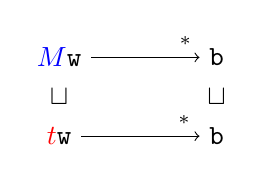
\begin{tikzpicture}[node distance=30mm, auto, transform 
		shape]
		\node (p) at (0,0) {$\Tm\wo$};
		\node (q) at (2,0) {$\bool$};
		\node (w) at (0,-1) {$\tm\wo$};
		\node (r) at (2,-1) {$\bool$};
		\node at (0,-0.5) {$\vappr$};
		\node at (2,-0.5) {$\vappr$};
		\draw (q) edge[<-] node [very near start, above=-3pt] {$^*$} (p);
		\draw (r) edge[<-] node [very near start, above=-3pt] {$^*$} (w);
		\end{tikzpicture}
	\end{center}
	This is particularly interesting if one thinks of $\Tm$ as a term that decides a language $\lan\subseteq\Sigma^*$.
	\begin{definition}
		$\Tm$ decides a language $\lan$ when $\Tm:\Str\to\Bool$ and $\Tm\wo\topcf^*\one$ if and only if $\wo\in\lan$.
	\end{definition}
	Indeed, for every word $\wo$ there exists a term $\tm^{\Tm}_\wo$ that simulates $\Tm$ when applied to $\wo$. This way, one approximates $\Tm$ by way of a family of terms $\{\tm^{\Tm}_\wo\}_{\wo\in\Sigma^*}$. 
	It is quite easy to realize that the above diagram can be made quantitative. Indeed, simulating each $\topcf$ steps requires a constant numeber of $\toaff$ steps. Moreover, the process of \emph{pullback} produces \emph{linear} terms. This means that the size of the approximant of $\Tm$ is bounded by the length of the reduction of $\Tm$.
	\begin{theorem}
		The following quantitative diagram holds, and moreover, $\size{\tm}=\bigo(\fun(\size{\wo}))$.
		\begin{center}
			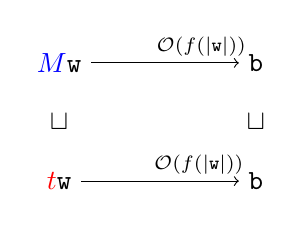
\begin{tikzpicture}[node distance=30mm, auto, transform 
			shape]
			\node (p) at (0,0) {$\Tm\wo$};
			\node (q) at (2.5,0) {$\bool$};
			\node (w) at (0,-1.5) {$\tm\wo$};
			\node (r) at (2.5,-1.5) {$\bool$};
			\node at (0,-0.75) {$\vappr$};
			\node at (2.5,-0.75) {$\vappr$};
			\draw (q) edge[<-] node [near start, above=-3pt] {$^{\bigo(\fun(\size{\wo}))}$} (p);
			\draw (r) edge[<-] node [near start, above=-3pt] {$^{\bigo(\fun(\size{\wo}))}$} (w);
			\end{tikzpicture}
		\end{center}
	\end{theorem}
	An important measure that will be useful in the following is the rank of an approximant.
	\begin{definition}
		The function $\rk:\Aff\to\mathbb{N}$ is defined in the following way by induction on the structure of approximant terms.
		\[\begin{array}{lll}
			\rk(\var)=0 & \rk(\la{\bag{\var_1\ldots\var_n}}\tm)=\rk(\tm) & \rk(\tm\tmtwo)=\max\{\rk(\tm),\rk(\tmtwo)\}\\[4pt]
			\rk(\bag{\tm_1\ldots\tm_n})=n & \ldots
		\end{array}\]
	\end{definition}
	\begin{proposition}
		For any term $\tm$, $\rk(\tm)\leq\size{\tm}$.
	\end{proposition}
	The maximum rank $\mrk^{\Tm}_n$ for a family of terms $\{\tm_{\wo}^{\Tm}\}_{\size{\wo}=n}$
	\[
	\mrk^{\Tm}_n=\max_{\size{\wo}=n}\rk\:\tm^{\Tm}_{\wo}
	\]
	clearly is still $\bigo(\fun(\size{\wo}))=\bigo(\fun(n))$.
	
	The idea now is that we can switch from terms $\tm_{\wo}^{\Tm}$ that approximate $\Tm$ on just one input word $\wo$ to terms $\tmtwo_{n}^{\Tm}$ that approximate $\Tm$ for every word $\wo$ such that $\size\wo=n$. In particular, for each term $\Tm$ it is possible to derive a family of \emph{canonical} approximations $\appfam{\Tm}{\mrk}$ such that the followings hold:
	\begin{itemize}
		\item $\size{\appfam{\Tm}{\mrk}}=\poly(\mrk)$;
		\item if $\tm\appr\Tm$ and $\rk\:\tm\leq\mrk$, then $\tm\appraff\appfam{\Tm}{\mrk}$.
	\end{itemize}
	Now, since $h:=\mrk^{\Tm}_n=\bigo(\fun(n))$, it is possible to approximate the family $\{\tm_{\wo}^{\Tm}\}_{\size{\wo}=n}$ by $\appfam{\Tm}{h}$, whose size is $\size{\appfam{\Tm}{h}}=\bigo(\poly(\fun(n)))$. The main point is that $\appfam{\Tm}{h}$ is easily computable.
	\begin{definition}
		We define as $\ltime(\fun(n))$ the class of languages that can be recognised by a $\pcf$-term $\Tm$ in at most $\fun(n)$ steps, where $n$ is the size of the input.
	\end{definition}
	\begin{theorem}
		$\ltime(\fun(n))\subseteq\dtime(\poly(\fun(n)))$.
	\end{theorem}
	\begin{proof}
		If $\Tm\in\ltime(\fun(n))$, then it can be \emph{easily} approximated by a family of approximations $\appfam{\Tm}{h}$ such that $\size{\appfam{\Tm}{h}}=\bigo(\poly(\fun(n)))$. Now, since $\appfam{\Tm}{h}$ is affine, it can be executed on a Turing machine in $\bigo(\poly(\fun(n)))$ steps.
	\end{proof}
	
	
	
	
%	\begin{theorem}[Monotonicity]
%		If $\tm\toaff\tmtwo$ and $\tm\appraff\tm'$, then $\tm'\toaff\tmtwo'$ such that $\tmtwo\appraff\tmtwo'$.
%	\end{theorem}
\begin{figure}
	\[
	\begin{array}{rcl}
	\multicolumn{3}{c}{\textsc{Call-by-Value PCF Terms, Values and Contexts}}\\[5pt]
	\Tm,\Tmtwo&\grameq&\Var\in\mathcal{V} \grampipe \La\Var\Tm \grampipe \Tm\Tmtwo  \grampipe \wo\in\Sigma^*\grampipe \isempty\Tm\grampipe\cons\Tm\Tmtwo\grampipe\\
	&&\bool\in\{\zero,\one\}\grampipe \ite\Tm\Tmtwo\Tmthree \grampipe \Fix\F\Tm\\[3pt]
	\Va&\grameq&\Var\in\mathcal{V}\grampipe\La\Var\Tm \grampipe\wo\in\Sigma^*\grampipe\bool\in\{\zero,\one\}\\[3pt]
	\Ctx&\grameq&\Hole\grampipe\Ctx\Tmtwo\grampipe\Va\Ctx\grampipe\isempty\Ctx\grampipe\cons\Ctx\Tmtwo\grampipe\cons\Va\Ctx\grampipe\ite\Ctx\Tmtwo\Tmthree
	\end{array}
	\]
	\[
	\begin{array}{rcl}
	\multicolumn{3}{c}{\textsc{Reduction Rules at Top Level}}\\[5pt]
	(\La\Var\Tm)\Va&\tlpcf&\Tm\isub\Var\Va\\
	\isempty\Ems&\tlpcf&\one\\
	\isempty\wo&\tlpcf&\zero\qquad\textrm{if }\wo\neq\Ems\\
	\cons\wo\wotwo&\tlpcf&\wo\wotwo\\
	\ite\one\Tm\Tmtwo&\tlpcf&\Tm\\
	\ite\zero\Tm\Tmtwo&\tlpcf&\Tmtwo\\
	\Fix\F\Tm&\tlpcf&\Tm\isub{\F}{\La\Var(\Fix\F\Tm)\Var}
	\end{array}
	\]
	\[
	\begin{array}{c}
	\textsc{Contextual Closure}\\[5pt]
	\infer{\Ctxp\Tm\topcf\Ctxp\Tmtwo}{\Tm\tlpcf\Tmtwo}
	\end{array}
	\]
	\[
	\begin{array}{rcl}
	\multicolumn{3}{c}{\textsc{Types and Judgments}}\\[5pt]
	\Ty,\Tytwo&\grameq&\Str\grampipe\Bool\grampipe\Ty\to\Tytwo
	\end{array}
	\]
\end{figure}

\begin{figure}
	\[
	\begin{array}{rcl}
	\multicolumn{3}{c}{\textsc{Affine Approximant Terms}}\\[5pt]
	\tm,\tmtwo&\grameq&\var\in\mathcal{V} \grampipe \la{\bag{\var_1\ldots\var_n}}\tm \grampipe \tm\tmtwo  \grampipe \bag{\tm_1\cdots\tm_n}\grampipe \wo\in\Sigma^*\grampipe \isempty\tm\grampipe\cons\tm\tmtwo\grampipe\\
	&&\bool\in\{\zero,\one\}\grampipe \ite\tm\tmtwo\tmthree\\[3pt]
	%\Va&\grameq&\Var\in\mathcal{V}\grampipe\La\Var\Tm \grampipe\Wo\in\Sigma^*\grampipe\Zero\grampipe\One\\[3pt]
	%\Ctx&\grameq&\Hole\grampipe\Ctx\Tmtwo\grampipe\Va\Ctx\grampipe\Isempty\Ctx\grampipe\Cons\Ctx\Tmtwo\grampipe\Cons\Va\Ctx\grampipe\Ite\Ctx\Tmtwo\Tmthree
	\end{array}
	\]
	\[
	\begin{array}{rcl}
	\multicolumn{3}{c}{\textsc{Reduction Rules at Top Level}}\\[5pt]
	\multicolumn{3}{c}{\cdots}\\
%	(\La\Var\Tm)\Va&\tlpcf&\Tm\isub\Var\Va\\
%	\Isempty\Ems&\tlpcf&\One\\
%	\Isempty\Wo&\tlpcf&\Zero\qquad\textrm{if }\Wo\neq\Ems\\
%	\Cons\Wo\Wotwo&\tlpcf&\Wo\Wotwo\\
%	\Ite\One\Tm\Tmtwo&\tlpcf&\Tm\\
%	\Ite\Zero\Tm\Tmtwo&\tlpcf&\Tmtwo\\
%	\Fix\F\Tm&\tlpcf&\Tm\isub{\F}{\La\Var(\Fix\F\Tm)\Var}
	\end{array}
	\]
	\[
	\begin{array}{c}
	\textsc{Contextual Closure}\\[5pt]
	\cdots%\infer{\Ctxp\Tm\topcf\Ctxp\Tmtwo}{\Tm\tlpcf\Tmtwo}
	\end{array}
	\]
	\[
	\begin{array}{rcl}
	\multicolumn{3}{c}{\textsc{Types and Judgments}}\\[5pt]
	\ty,\tytwo&\grameq&\Str\grampipe\Bool\grampipe\ty\to\tytwo\grampipe \bag{\ty_1\cdots\ty_n}
	\end{array}
	\]
\end{figure}

\begin{figure}
	\[
	\begin{array}{rcl}
	\multicolumn{3}{c}{\textsc{Approximation Relation }\appr}\\[5pt]
	\multicolumn{3}{c}{\cdots}\\
	\end{array}
	\]
\end{figure}

\begin{figure}
	\[
	\begin{array}{rcl}
	\multicolumn{3}{c}{\textsc{Affine Approximants Relation }\appraff}\\[5pt]
	\multicolumn{3}{c}{\cdots}\\
	\end{array}
	\]
\end{figure}

\end{document}